% arara: pdflatex
% !arara: biber
% !arara: pdflatex
% How to run: 
% 1) pdflatex "filename".tex
% 2) biber "filename"
% 3) pdflatex "filename".tex
% 4) pdflatex "filename".tex


\documentclass[x11names]{article}
\usepackage{verbatim}
\usepackage{listings}
\usepackage{graphicx}
\usepackage{color}
\usepackage{amsmath}
\usepackage{amssymb}
\usepackage[T1]{fontenc}
\usepackage{shadow}
\usepackage{hyperref}
\usepackage{physics}
\usepackage{url}
%For use in pictures
\usepackage{tikz}
\usepackage{tikz-3dplot}
\usepackage{wrapfig}

\usepackage[l2tabu]{nag} %NAgs when using bad practices


\usepackage{subcaption}
\usepackage[utf8]{inputenc}
\usepackage{booktabs} % Allows the use of \toprule, \midrule and \bottomrule in tables
\usepackage[font={small,it}]{caption}
\usepackage[margin=0.7in]{geometry} %Sets the margins in the document
\usepackage{siunitx}    %Allows use of SI units macros

%Defines calculator way to write powers of ten
\sisetup{output-exponent-marker=\textsc{e}}


% Change numbering and some commands
\renewcommand\thesection{Exercise \Roman{section}}
\renewcommand\thesubsection{\Roman{section}.\alph{subsection}}

%% references
\usepackage[style=authoryear,
            bibstyle=authoryear,
            backend=biber,
            % refsection=chapter,
            maxbibnames=99,
            maxnames=2,
            firstinits=true,
            uniquename=init,
            natbib=true,
            dashed=false]{biblatex}

\addbibresource{bibliography.bib}

\usepackage[capitalize]{cleveref}

\setcounter{tocdepth}{2}

\lstset{language=c++}
\lstset{alsolanguage=[90]Fortran}
\lstset{basicstyle=\small}
\lstset{backgroundcolor=\color{white}}
\lstset{frame=single}
\lstset{stringstyle=\ttfamily}
\lstset{keywordstyle=\color{red}\bfseries}
\lstset{commentstyle=\itshape\color{blue}}
\lstset{showspaces=false}
\lstset{showstringspaces=false}
\lstset{showtabs=false}
\lstset{breaklines}


\definecolor{keywords}{RGB}{255,0,90}
      \definecolor{comments}{RGB}{0,0,113}
      \definecolor{red}{RGB}{160,0,0}
      \definecolor{green}{RGB}{0,150,0}
       
      \lstset{language=Python, 
              basicstyle=\ttfamily\small, 
              keywordstyle=\color{keywords},
              commentstyle=\color{comments},
              stringstyle=\color{red},
              showstringspaces=false,
              identifierstyle=\color{green}
              }



\title{ Exercise 9 \\ Sommerjobb Numeriske Plasmaoppgaver }
\author{Gullik Vetvik Killie
		}

\renewcommand{\va}{\vec}

%%%%%%%%%%%%%%%%%%%%%%%%%%%%%%%%%%%%%%%%%%%%%%%%%%%%%%%%%%%%%%%%%%%%%%%%%%%%%%%%%%%%
% Actual text starts here
%%%%%%%%%%%%%%%%%%%%%%%%%%%%%%%%%%%%%%%%%%%%%%%%%%%%%%%%%%%%%%%%%%%%%%%%%%%%%%%%%%%%
\begin{document}


\maketitle

\section{}

\subsection{Theory}
  In this exercise we will investigate how electrically charged particles behave in the converging magnetic field above the north pole. We will especially consider the stability case where there is a balance between the magnetic moment force and gravity.
\\ \\
  A particle gyrating in a magnetic field \(B\) will have a magnetic moment given by

  \begin{align}
    \va{\mu} &= \frac{mv_\perp^2}{2B} \va{e}_B
  \end{align}

  \noindent The gradient force felt by the particle is then given by

  \begin{align}
    \va{F}_B &= -\left( \va{\mu}\cdot\nabla \right)\va{B}
  \end{align}

  \noindent The particle will also feel a gravitational force and we will consider te case those two forces are in balance, so the sum of forces on the particle is constant.

  \begin{align}
    -\va{F}_G + \va{F}_B &= 0  
    \\
    mg(z) &= \frac{mv_\perp^2}{2B(z)} \pdv{B_z(z)}{z}
  \end{align}

  \noindent If we let the magnetic field be approximated as in the previous exercises,

  \begin{align}
    \va{B}(\va{r}) &= \frac{\mu_0}{4\pi}\left( \frac{3\va{r}(\va{r}\cdot\va{m}  )}{r^5} - \frac{\va{m}}{r^3} \right)
    \intertext{and the gravitational acceleration is given by }
    \va{g}(\va{r}) &= - \gamma \frac{M_e}{r^3}
      \begin{pmatrix}
        x \\ y \\ z
      \end{pmatrix}
    \intertext{The equation of motion for the particle is then given by}
    m\pdv{\va{v}}{t} &= q \va{v}\cross\va{B} + m\va{g}
  \end{align}

  \noindent Let us consider the case where the particle is \(200 \si{\kilo\meter}\) straight above the magnetic north, so the guiding center coordinates is
  \( \va{r}_0 = (0,0,200\si{\kilo\meter} + R_e)\). Then it becomes simpler to find the z directed part of the gradient.

  \begin{align}
    \pdv{B_z(z)}{z} &= \pdv{}{z}\left( \frac{\mu_0}{4\pi} \left(\frac{3z^2m_z}{z^5} - \frac{m_z}{z^3} \right)\right)
    \\
    &= \frac{\mu_0m_z}{4\pi} \left( - \frac{9}{z^4} + \frac{3}{z^4} \right)
    \\
    &= - \frac{3\mu_0m_z}{2\pi z^4}
  \end{align}

  \noindent Then the gyration velocity giving a balance in the force given by:

  \begin{align}
    v^2_\perp &=  2B(z)g(z) \left(\pdv{B_z(z)}{z} \right)^{-1}
    \intertext{inserting the numbers we get an initial velocity of}
    v_\perp &\approx 6300 \si{\meter\per\second}
  \end{align}

  \noindent We will now solve the equation of motion for the electron using runge-kutta-4 as the time integrator, we follow the same algorithm as in exercise 3.
  

\subsection{Results}
  \subsection{Error analysis}

    \begin{figure}
      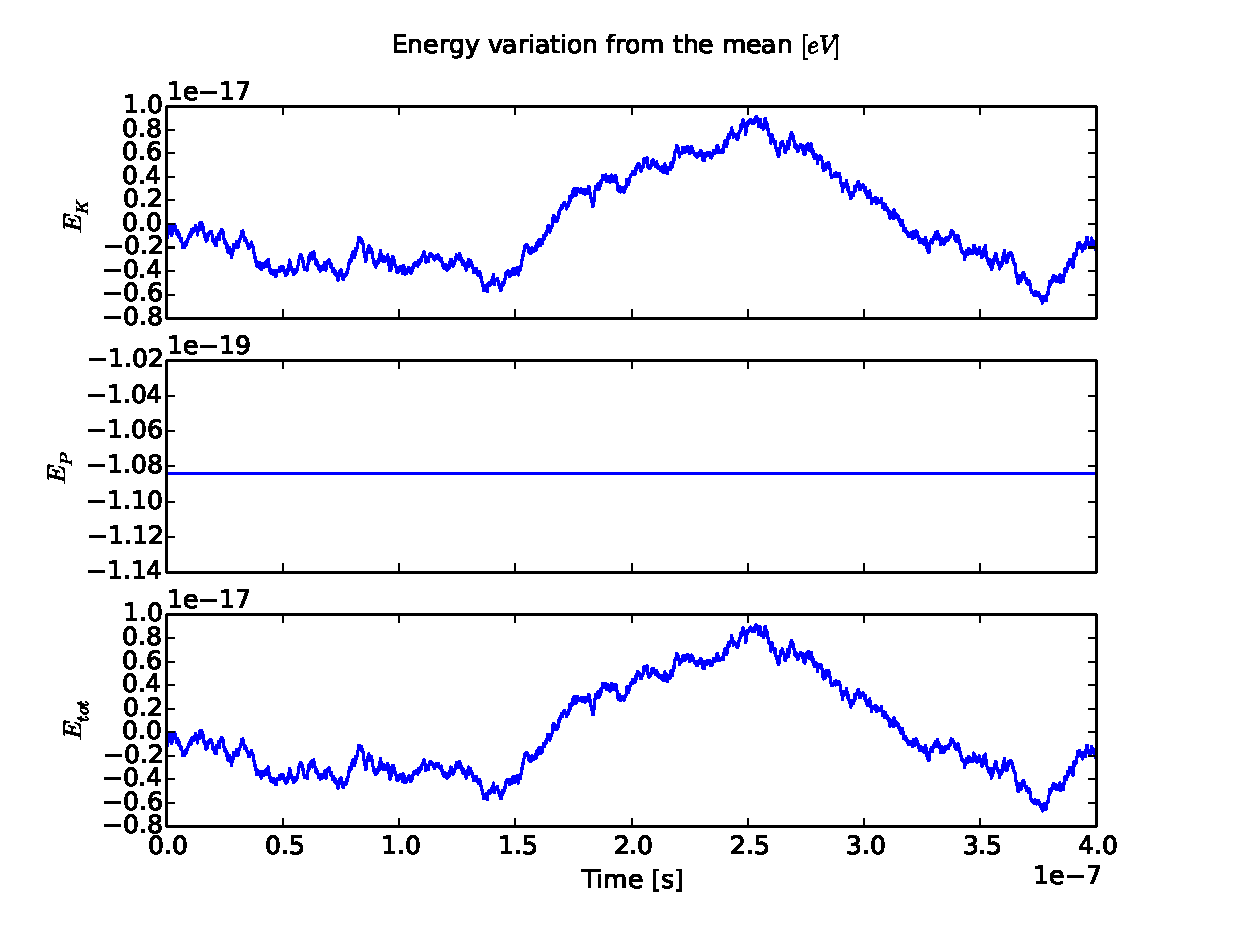
\includegraphics[width = 0.5\textwidth]{figures/6-0/energy}
      \caption{The variation of the energy around the mean was measured for the case when the electron was in balance with no vertical velocity. Then mean kinetic energy, potential energy and total energy was respectively \(E_K = 1.135\times 10^{-4}eV\), \(E_P = -3.406\times 10^{-4} eV\) and  \(E_{tot} = -2.271\times 10^{-4} eV\)}
      \label{fig:energy}
    \end{figure} 

    To check how trustworthy the results are we calculated the energy. Since the energy of the particle is conserved, and given by \(E_{tot} = E_K + E_P = \frac{mv^2}{2} + mgz\). The energy of the particle is not dependent on the magnetic field since it can do no work on the particle. After testing a few differing timesteps, with no vertical velocity, we arrived at \(10^{-10}\si{\second}\) at which the energy didn't have a systematic error, see \cref{fig:energy}.


  \subsection{Results}
  \begin{figure}
      \centering
      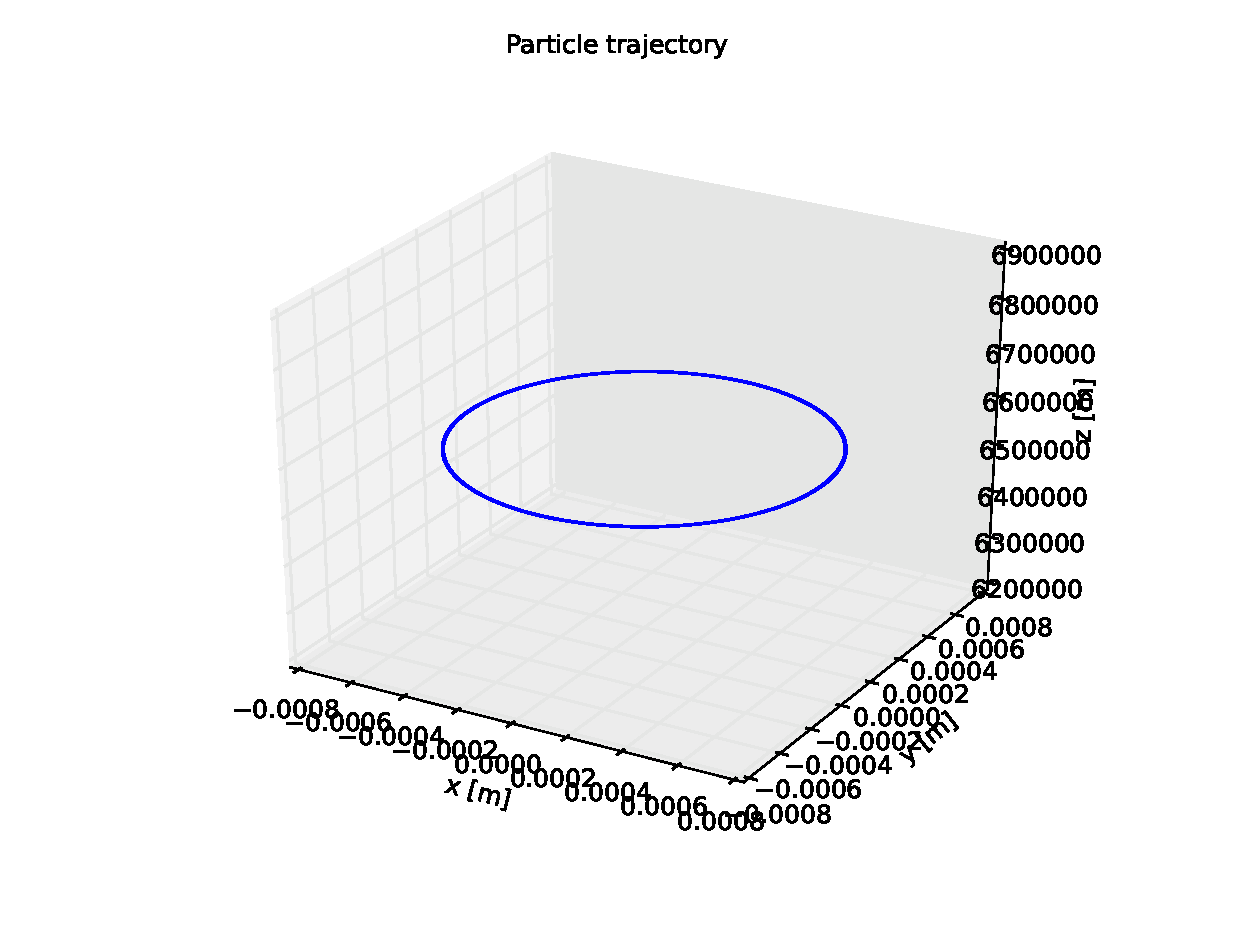
\includegraphics[width = 0.30\textwidth]{figures/6-0/3Dplot}
      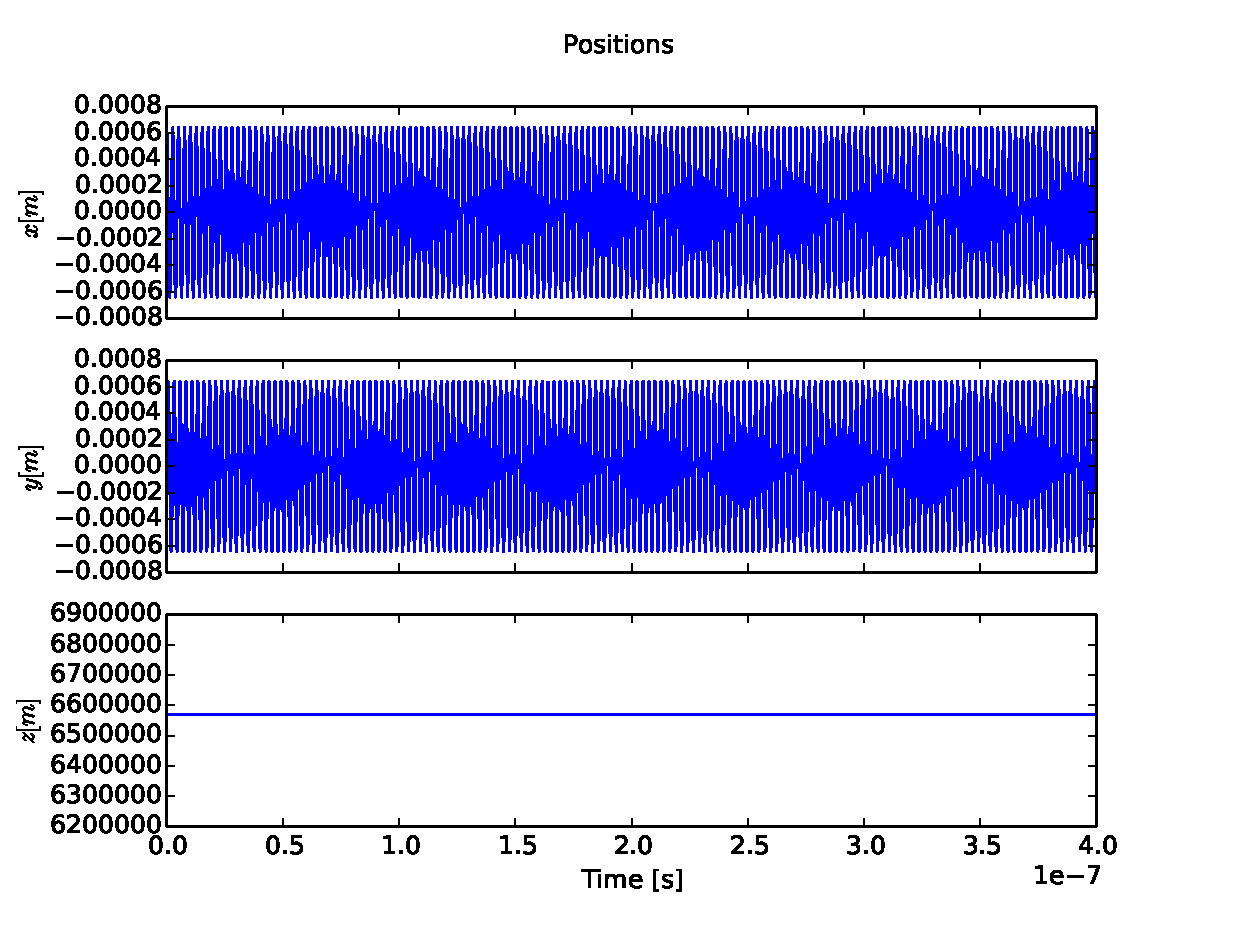
\includegraphics[width = 0.30\textwidth]{figures/6-0/xyz}
      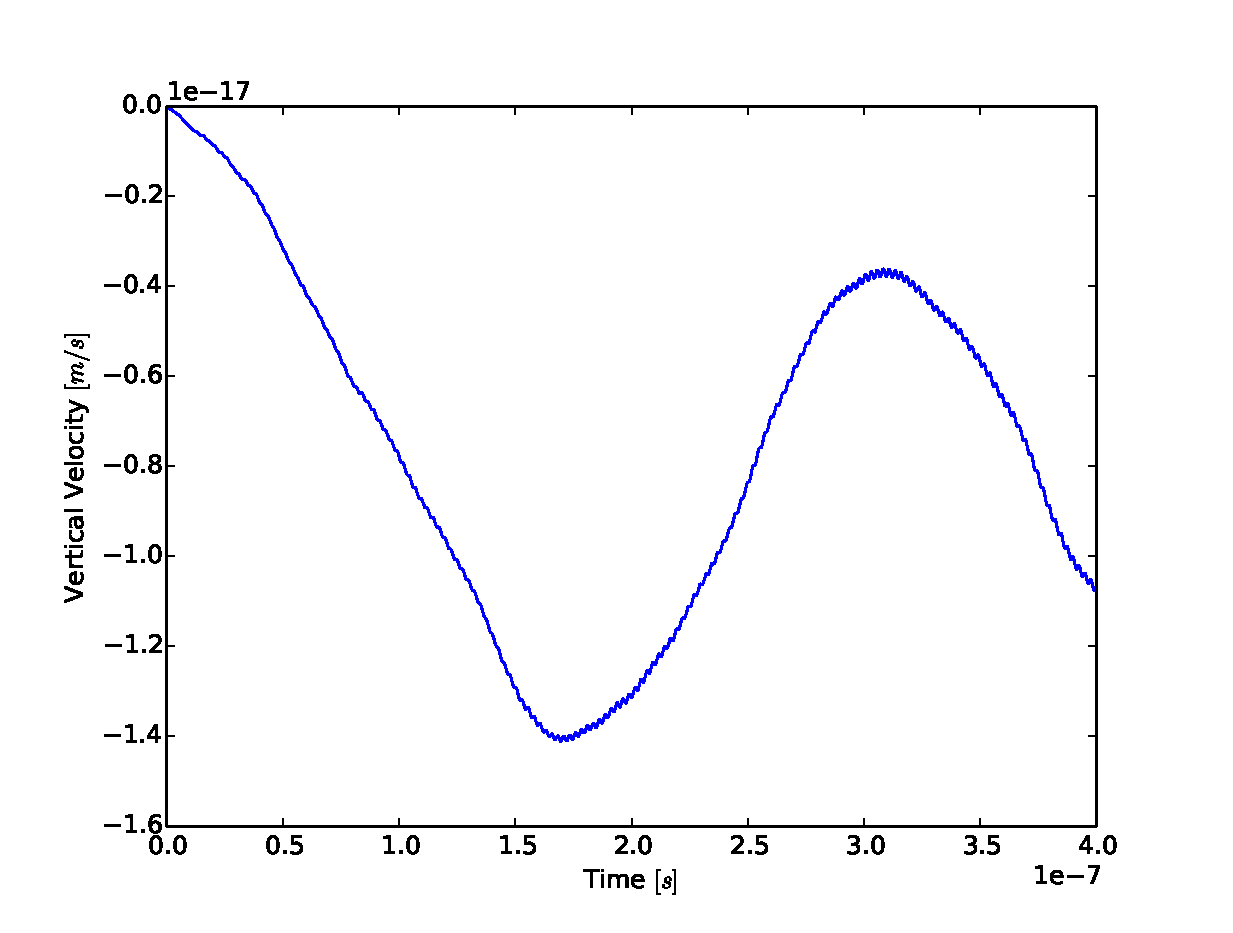
\includegraphics[width = 0.30\textwidth]{figures/6-0/vertical_vel}
      \caption{The figures show a particle in the gyrating above the north pole, with a perpendicular velocity causing the gravitational and magnetic gradient force to balance. The figure to the left shows the position, the center figure shows the positions as xyz coordinates and the figure to the right shows the vertical velocity. This particle had }
      \label{fig:no_perturbation}
    \end{figure}

  We first started the particle with a perpendicular velocity which had a balance between the magnetic gradient force and the gravitational force, so the vertical force the particle feels will be \(0\) and the particle will gyrate around the starting point. This can be seen in \cref{fig:no_perturbation} although there is a small change in the vertical velocity, which is probably due to some numerical inaccuracy, or that the initial velocity is slightly off due to the particle being a gyration radius to the side of the magnetic north.

  \begin{figure}
      \centering
       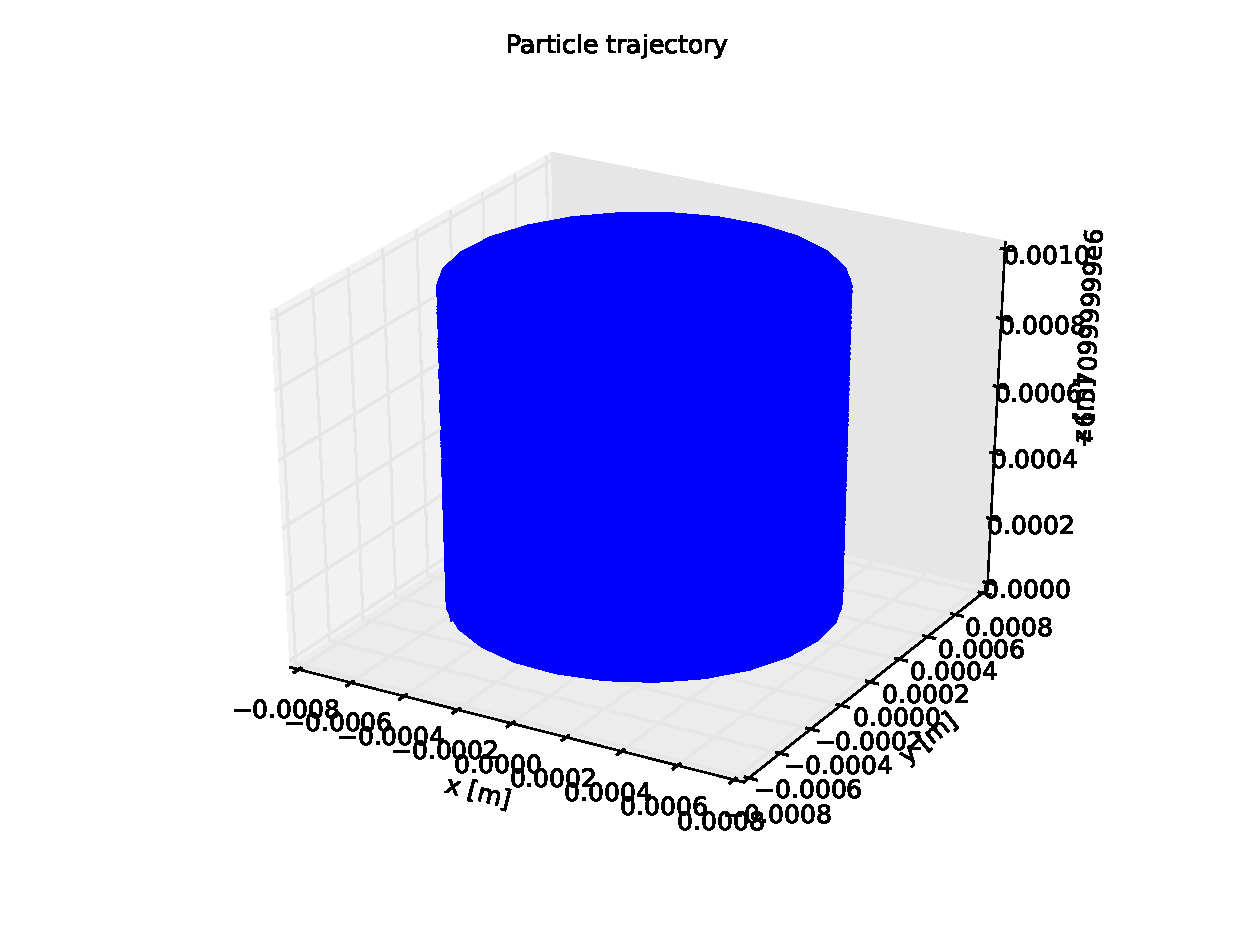
\includegraphics[width = 0.30\textwidth]{figures/6--5/3Dplot}
      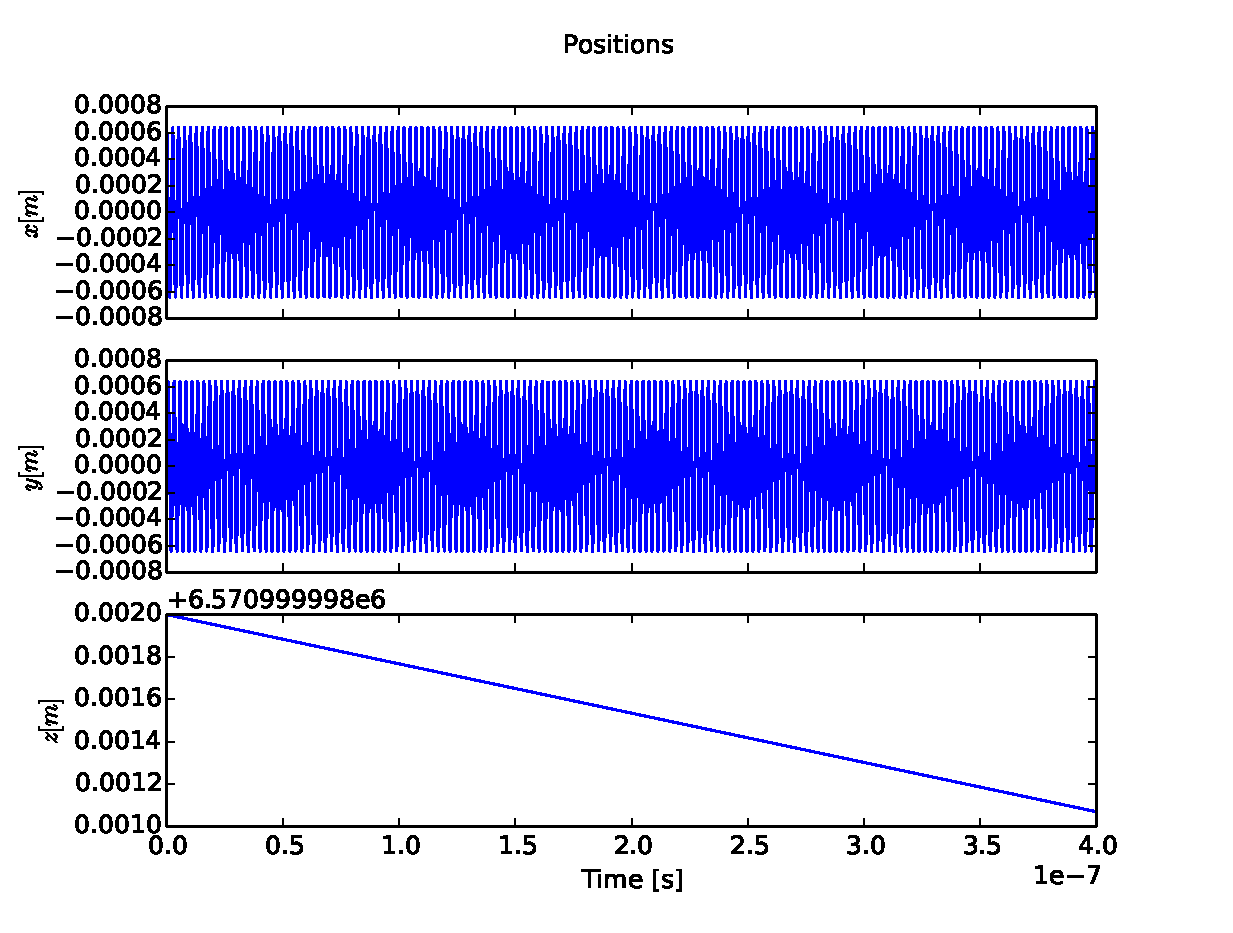
\includegraphics[width = 0.30\textwidth]{figures/6--5/xyz}
      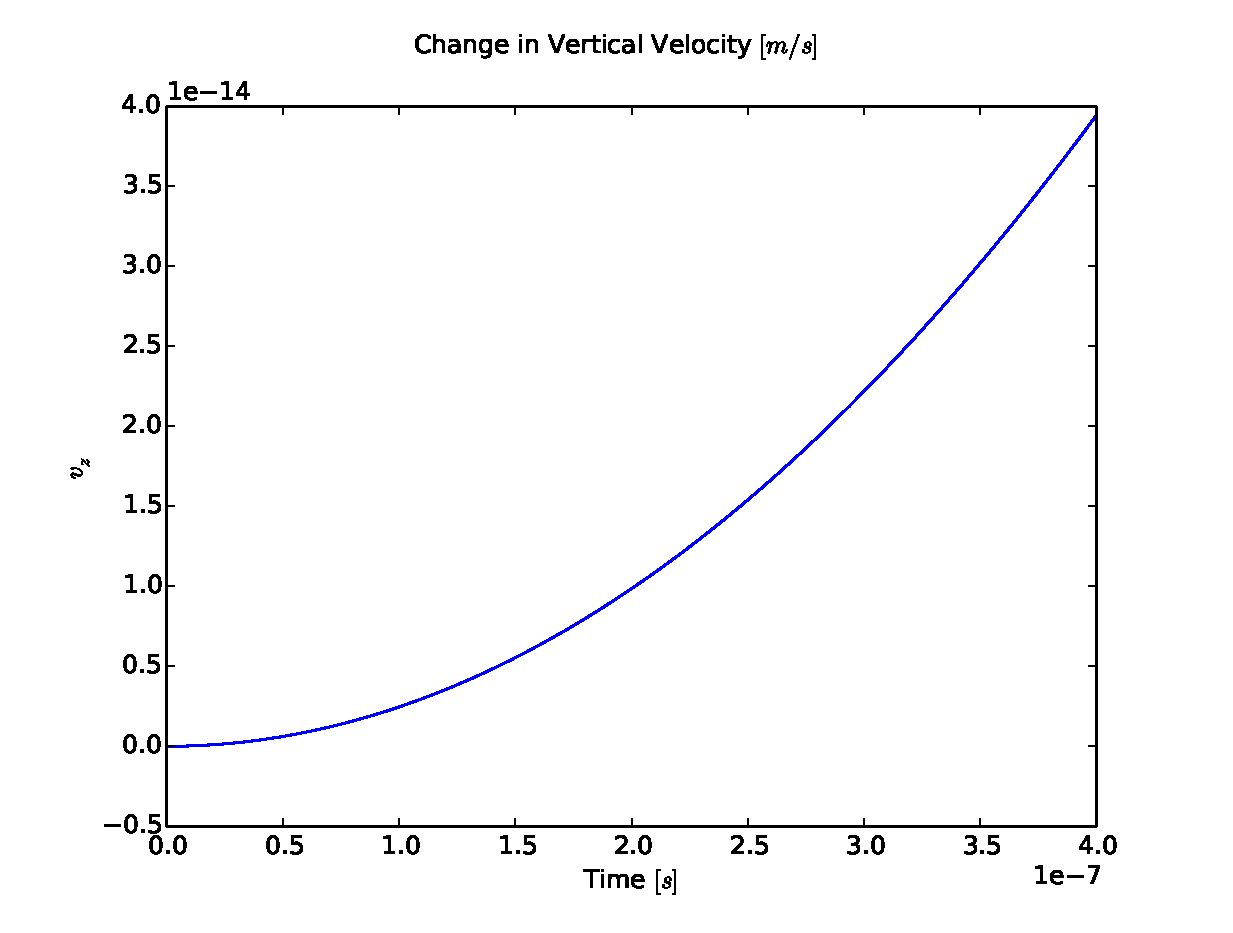
\includegraphics[width = 0.30\textwidth]{figures/6--5/vertical_vel}
       \caption{ This particle started with a slight velocity toward the towards the earth of \(5 \si{\meter\per\second}\). The figure to the shows the position, the center figure shows the positions as xyz coordinates and the figure to the right shows the change in the vertical velocity. The change in the vertical velocity is positive which indicates that it will eventually cause the particle to move upwards again, indicating a that the initial position is a stable position.}
      \label{fig:down_perturbation}
    \end{figure}

  \begin{figure}
      \centering
      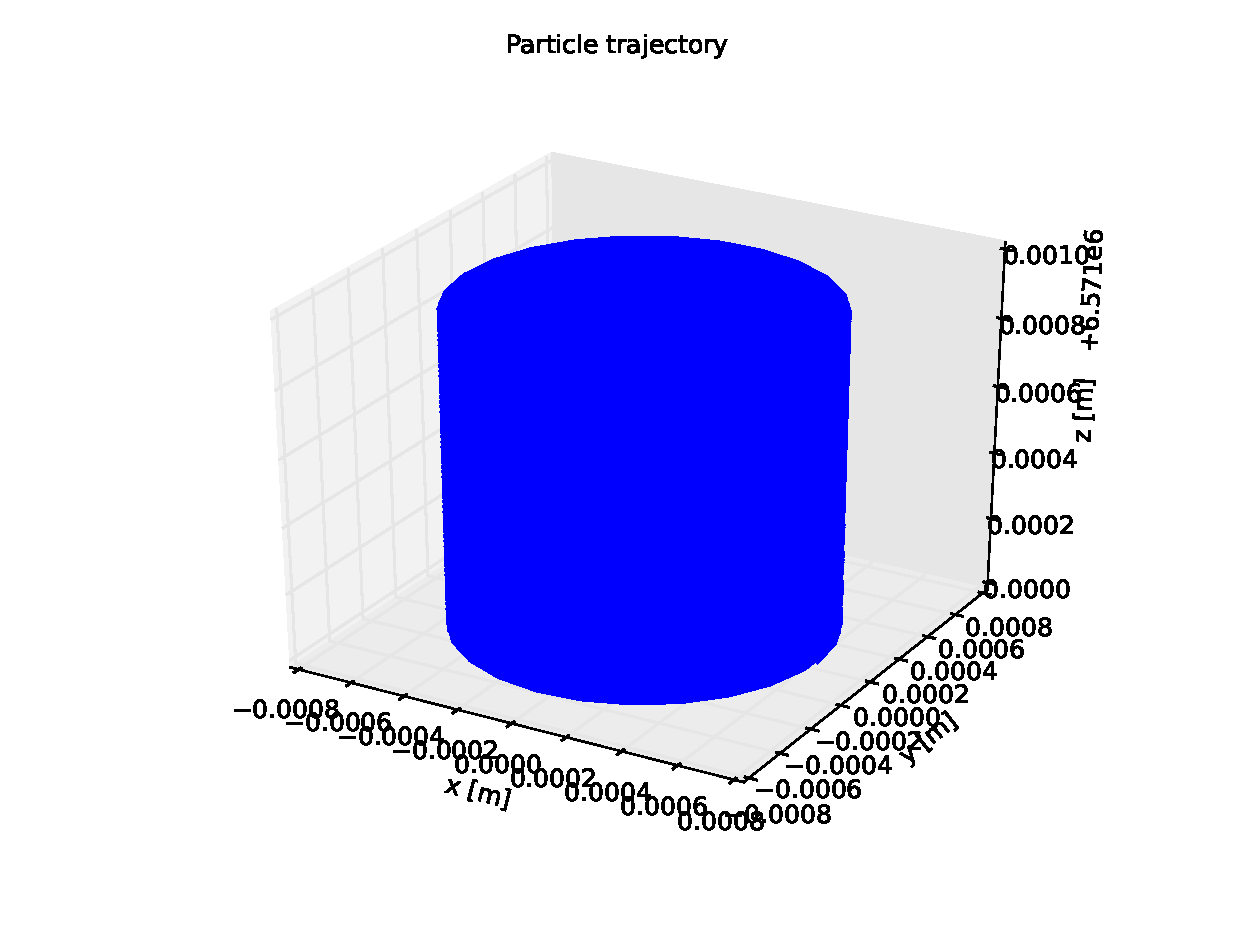
\includegraphics[width = 0.30\textwidth]{figures/6-5/3Dplot}
      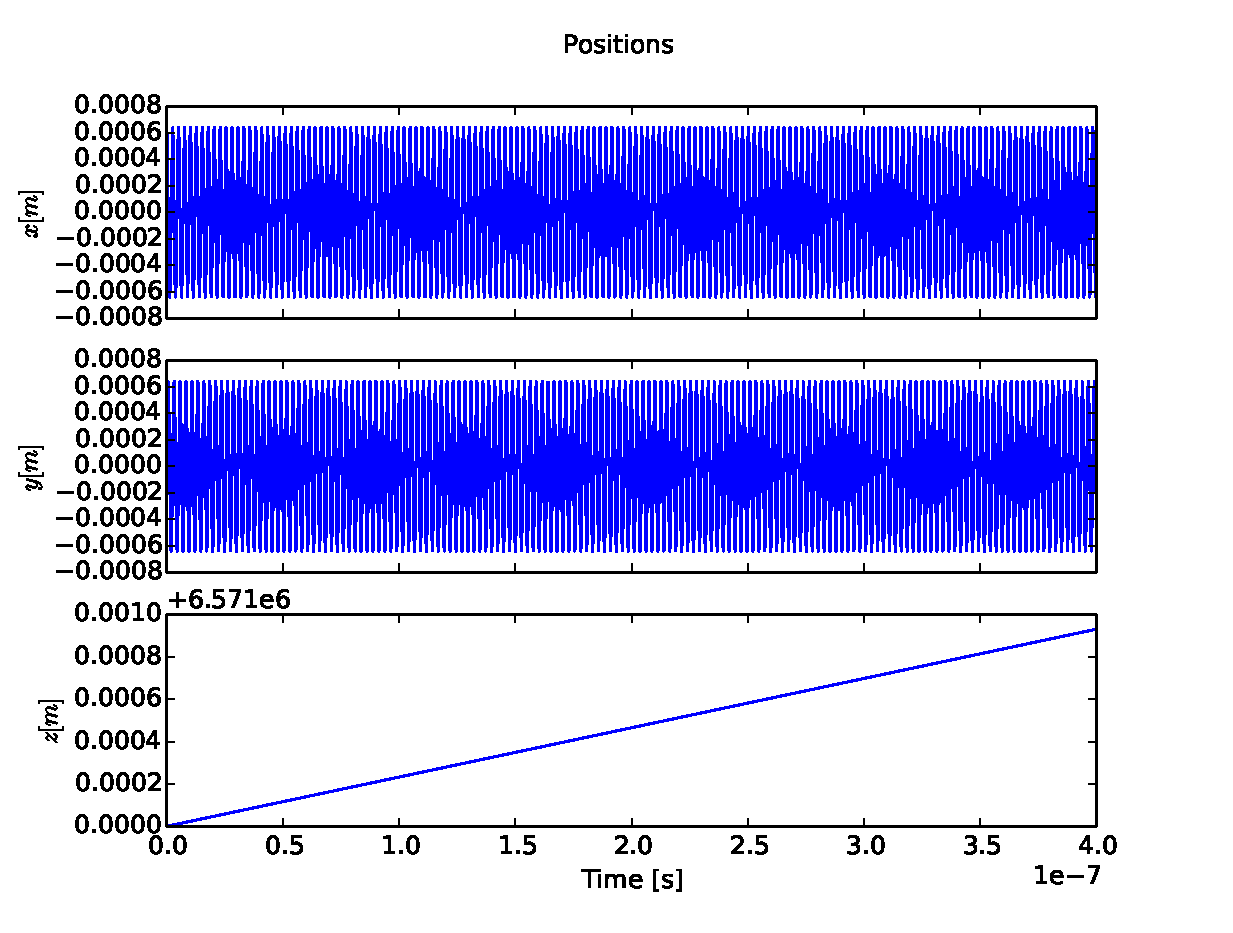
\includegraphics[width = 0.30\textwidth]{figures/6-5/xyz}
      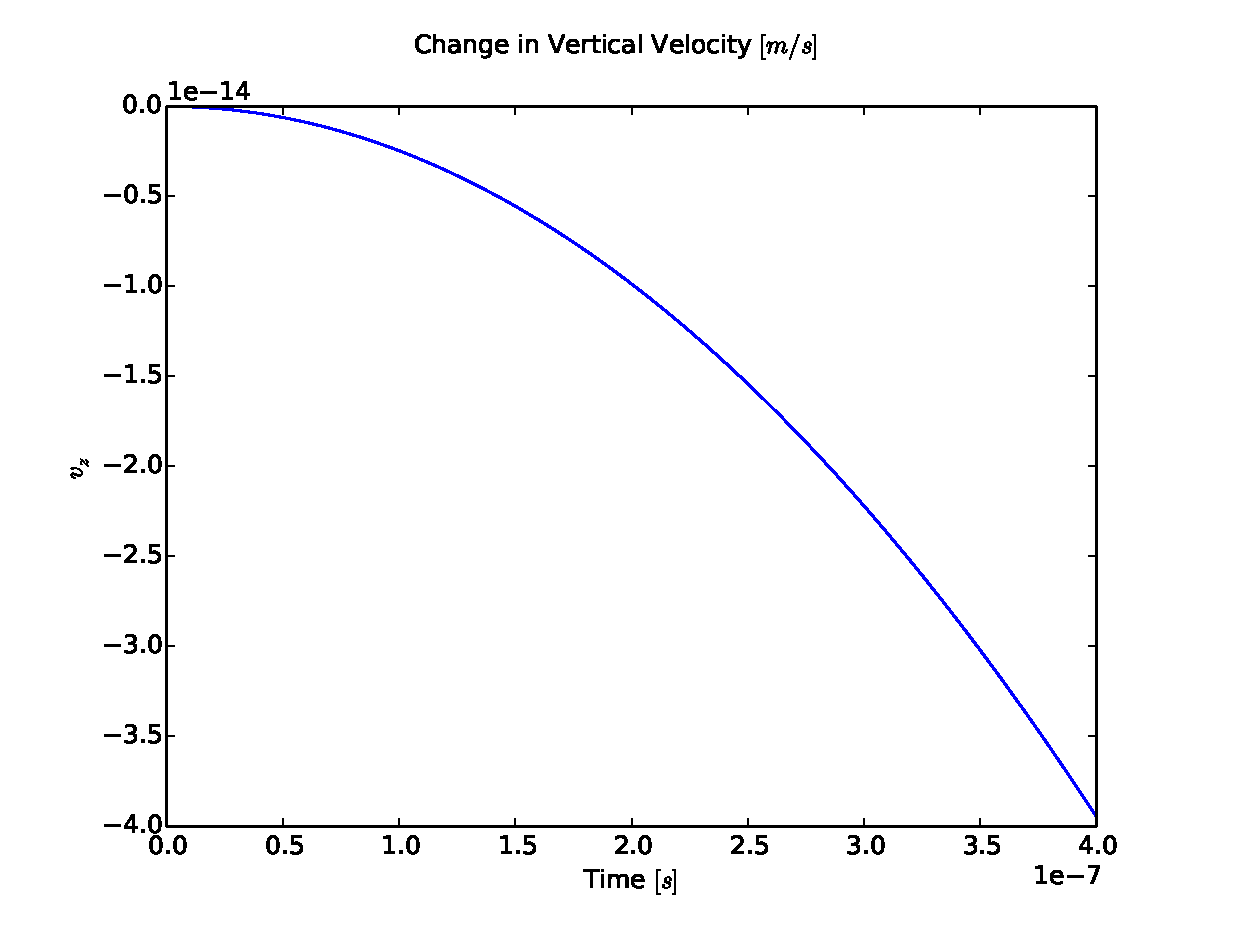
\includegraphics[width = 0.30\textwidth]{figures/6-5/vertical_vel}
      \caption{ This particle started with a slight velocity away from the earth of \(5 \si{\meter\per\second}\). The figure to the shows the position, the center figure shows the positions as xyz coordinates and the figure to the right shows the change in vertical velocity. The change in the vertical velocity indicates that the particle will eventually begin moving toward the initial position again indicating that the initial positions was a stable position.}
      \label{fig:up_perturbation}
   \end{figure}

  \cref{fig:down_perturbation,fig:up_perturbation} shows a particle with a slight downward velocity of \(5 \si{\meter\per\second}\), and the same upward velocity, which will cause the particle to move out the height at which the magnetic gradient force and the gravitational force will balance. As the particle begins to move downward gravitational force pulling it down will increase. In addition the gradient of the magnetic force will also increase. Since the particle has a positive change in \(v_z\) when \(v_z < 0\) and a negative change in the opposite case, there particle will move towards the initial position again in both cases. Unfortunately we couldn't simulate the particle for a long enough time for it to do the expected oscillation around the initial position to see if the oscillation would remain stable.

\appendix

\section{Comments}
  \begin{itemize}
    \item I spoke to some students and everyone should be quite familiar with RK4 by the third year, so it should be done. Maybe it would be better to start RK4 in exercise 2, since it is a quite short exercise and then they won't have to write new code for exercise 3 which is quite abit more extensive.
    \item In the text it's written that the particle should be placed \(\frac{1}{2}\) a gyro radius to the side of magnetic pole. I assume we want to place the guiding center of the particle at the magnetic pole, which would need the particle to be placed \(1\) gyro radius to the side.
    \item Parenthesis around the magnetic field, equation \(5\).
    \item In equation \(6\) the equation of motion is listed as 
    \[m\pdv{\va{v}}{t} = q\va{v} \cross \va{B} - m \va{g}\]
    , and in equation \(7\) the gravity vector is listed as negative with respect to the direction.
    One of these should be positive so the gravitational force works the right direction (give a negative \(v_z\)).
    \item In the hint section the Earths mass has the wrong number, it should be to the power \(24\) instead of \(23\).
  \end{itemize}


\section{Boring manual calculation}
  Assuming that the particle is directly above the magnetic north pole, so the radius is given by the \(z\)-coordinate, the 3 factors become:
   \begin{align}
    \begin{split}
      B(z) &= \frac{\mu_0}{4\pi}\left( \frac{3z^2m_z}{z^5} - \frac{m_z}{z^3} \right) =  \frac{\mu_0 m_z}{2\pi z^3} \approx \frac{4\pi \times 10^{-7} \times 7.94 \times 10^{22}}{2\pi\times (6.571\times 10^6 \si{m})^3} \si{\tesla}\approx 5.597\times 10 ^{-5} \si{\tesla}
      \\
      g(z) &= - \gamma \frac{M_e}{z^3} z = -\frac{\gamma M_e}{z^2} \approx - \frac{6.7 \times 10^{-11} \times 5.9 \times 10^{24}}{(6.571\times 10^6 )^2} \si{\meter \per \second^2} \approx -9.1 \si{\meter\per\second^2}
      \\
      \pdv{B_z(z)}{z} &= - \frac{3\mu_0m_z}{2\pi z^4} \approx -\frac{6 \times 10^{-7}\times 7.94\times 10^{22}}{(6.571\times 10^6 )^4 } \si{\tesla \per\meter } \approx -2.55\times 10^{-11} \si{\tesla \per\meter }
    \end{split}
    \intertext{and the total initial perpendicular velocity will be}
    v_\perp &\approx \sqrt{ (5.597\times 10 ^{-5} \si{\tesla}) \times (-9.1 \si{\meter\per\second^2}) / (2.55\times 10^{-11} \si{\tesla \per\meter } )} \approx 6300 \si{\meter\per\second}
  \end{align}

\section{Code}
  \label{sec:code}
  \lstinputlisting{../source/stability.py}


\end{document}